\documentclass[twoside]{article}
\usepackage{color}
%\usepackage{enumerate}
\usepackage{graphicx}
\usepackage{color}
\usepackage[cmex10]{amsmath}
\usepackage{array}
\usepackage{float}
\usepackage[utf8]{inputenc} 
\usepackage[portuguese]{babel}
\usepackage[font=normalsize,format=plain,labelfont=bf,up,textfont=up,figurename=Figura,tablename=Tabela]{caption}
\usepackage{subcaption}
\usepackage[top=1in, bottom=1in, left=1.25in, right=1.25in]{geometry}
\usepackage{indentfirst}
\usepackage{fancyhdr}

%% LaTeX Draw
%
%\usepackage[usenames,dvipsnames]{pstricks}
%\usepackage{epsfig}
%\usepackage{pst-grad} % For gradients
%\usepackage{pst-plot} % For axes
%\usepackage[space]{grffile} % For spaces in paths
%\usepackage{etoolbox} % For spaces in paths
%\makeatletter % For spaces in paths
%\patchcmd\Gread@eps{\@inputcheck#1 }{\@inputcheck"#1"\relax}{}{}
%\makeatother

% Font packages
\usepackage{amssymb}
\usepackage{amsfonts}
\usepackage{steinmetz}
% Nice extra font package, e.g. \mathds{1}
\usepackage{dsfont}


% Use multiple rows when writing tables
\usepackage{multirow}
\usepackage{booktabs}
\usepackage{bigstrut}
    \setlength\bigstrutjot{3pt}

% Uncomment next line to make footnots per page
\usepackage{perpage}

% Uncoment next group of lines to create the table of contents for the PDF
\usepackage{hyperref}
\definecolor{darkblue}{rgb}{0,0,0.5}
\hypersetup{
    pdftitle={Trabalho 1},
    pdfauthor={Gabriel Pelielo},
    bookmarksnumbered=true,     
    bookmarksopen=true,         
    bookmarksopenlevel=1,       
    colorlinks=true,
    linkcolor=darkblue,
    filecolor=darkblue,  
    urlcolor=darkblue,  
    citecolor=darkblue,              
    pdfstartview=Fit,           
    pdfpagemode=UseOutlines,    % this is the option you were lookin for
    pdfpagelayout=TwoPageRight
}

\renewcommand{\title}{Trabalho 2}
\newcommand{\subtitle}{Introdução à Otimização}
\pagestyle{fancy}
\fancyhead[L]{\title}
\fancyhead[R]{\subtitle}
\fancyhead[C]{\thepage}
\fancyfoot[C]{}

\allowdisplaybreaks
\usepackage[printwatermark]{xwatermark}%\newwatermark[allpages,color=black,angle=45,scale=4,xpos=0,ypos=0]{\todo{RASCUNHO}}
\debugtrue
\renewcommand{\labelitemi}{\scalebox{0.8}[0.8]{$\bullet$}}
\newcommand{\tab}{\hspace{0.5cm}}

\begin{document}
\large
\begin{titlepage}
\begin{center}

% Upper part of the page. The '~' is needed because \\
% only works if a paragraph has started.

\includegraphics[width=0.15\textwidth]{logo.png}%~\\[0.5cm]

% Title
\rule{\linewidth}{0.5mm} \\[0.4cm]
{ \huge \bfseries \title \\[0.4cm] }
\rule{\linewidth}{0.5mm} \\[0.5cm]

\textsc{\Large \subtitle}\\[1.5cm]

% Author and supervisor
\begin{minipage}{0.4\textwidth}
\begin{flushleft} \large
\textbf{Alunos: \newline Cayo Valsamis \newline Gabriel Pelielo \newline Rafael Accácio \newline Rodrigo Moysés}\\
%NOME DOS ALUNOS

\end{flushleft}
\end{minipage}
\begin{minipage}{0.4\textwidth}
\begin{flushright} \large
\textbf{Professor:\newline Afonso Celso del Nero \newline \newline \newline} \\
%NOME DO PROFESSOR
\end{flushright}
\end{minipage}

\vfill

% Bottom of the page
{\large \today}

\end{center}
\end{titlepage}

\tableofcontents

\newpage

\mysection{Introdução}

O trabalho detalhado neste relatório se baseia em analisar métodos numéricos para realizar busca de mínimos de funções vetoriais. Foram implementados cinco métodos diferentes de localização de mínimos:

\begin{itemize}
	\item Método da Descida Máxima (ou gradiente)
	\item Método do Gradiente Conjugado
	\item Método de Newton
	\item Método de Newton Modificado
	\item Método de Quase Newton
\end{itemize}

Todos os métodos foram implementados na plataforma \textit{MATLAB}, através de um programa de interface gráfica usado para escolher o método desejado e inserir alguns valores necessários para executar a busca. O objetivo do trabalho foi comparar esses métodos de acordo com os quesitos de tempo de execução, número necessário de iterações e por fim qualificá-los de acordo com cada função inserida.

\mysection{Mínimos Quadrados}\label{sec:min_quad}

\begin{frame}[t]{Mínimos Quadrados}
	\begin{itemize}
	\item Minimizar Quadrado dos Resíduos
	\end{itemize}\pause
	\begin{equation}
min(\sum^n (\mathbf{f}(t_k,\omega_n,\zeta)-\mathbf{y}_k))
\end{equation}\pause
\begin{itemize}
	\item $n$ é o número de amostras.\pause
	\item $k$ é uma amostra.\pause
	\item $\mathbf{f}(t_k,\omega_n,\zeta)$ é a expressão da função de resposta no tempo k.\pause
	\item $t_k$ é o instante de tempo da k-ésima amostra.\pause
	\item $\mathbf{y}_k$ é o valor medido na amostra $k$.\pause
	\item $\omega_n$ e $\zeta$ são os parâmetros do sistema.
	\note<8>{ZETA}
	\end{itemize}
\end{frame}

\begin{frame}[t]{"Dividir e Conquistar"}
\only<1-2>{Iremos dividir em duas partes}
\begin{enumerate}
\item<1-2> Calcular a expressão $\sum_{i=1}^k (\mathbf{f}(t_k,\omega_n,\zeta)-\mathbf{y}_k)$\pause
\item<2> Minimizar a expressão através de algum método.
\end{enumerate}
\only<3>{\vspace{-1cm}Quais métodos?}
\only<4-6>{Métodos Antigos?\\}
\only<5-6>{ \vspace{1cm}\hspace{3cm}Métodos Novos?\\}
\only<6>{ \vspace{1cm}\hspace{6cm}Veremos...}
\end{frame}

\mysection{Algoritmo Genético}\label{sec:genetico}

\begin{frame}[t]{Algoritmo Genético}
	
	O algoritmo genético é inspirado pelo evolucionismo, que se baseia em gerações de indivíduos, em que os mais aptos prevalecem e constroem a geração futura.
	
	\begin{figure}[h]
		\begin{center}
			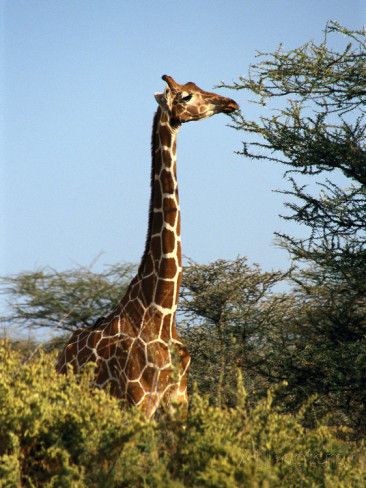
\includegraphics[width=3cm]{./giraffe.jpg}   
		\end{center}
	\end{figure}
	
\end{frame}

\begin{frame}[t]{Algoritmo Genético}
	
	O primeiro passo para a construção do algoritmo genético é a criação de uma \textbf{primeira geração}, feita aleatoriamente, com quantidade de indivíduos e limites definidos.
	
		\begin{center}
			\animategraphics[autoplay,loop,width=5cm]{1}{frame_}{1}{5}
		\end{center}
	
\end{frame}
	
\begin{frame}[t]{Algoritmo Genético}
	O segundo passo é criar a \textbf{população intermediária}. O método escolhido para tal foi o canônico, com aptidão definida como 
	
	\begin{equation*}
		\phi_i = \dfrac{\bar{f}}{f_i}
	\end{equation*}
	
	Sendo
	\begin{itemize}
		\item $ \phi_i $ a aptidão do indivíduo $ i $.
		\item $ f_i $ a função objetivo avaliada no ponto do indivíduo $ i $.
		\item $ \bar{f} $ a média do valor da função para toda a população.
	\end{itemize} 
	
\end{frame}

\begin{frame}[t]{Algoritmo Genético}
	
	O terceiro passo é a recombinação, processo necessário para construir a \textbf{segunda geração}. O tipo de recombinação escolhido foi a média de três pais, para acelerar a convergência.
	
	\begin{figure}[h]
		\begin{center}
		\begin{tikzpicture}[scale = 0.65]
		
		
		\draw  (-5.0,4.0) rectangle (-1.5,-2.5);
		\draw  (0.0,4.0) rectangle (3.5,-2.5);
		\draw  (5.0,4.0) rectangle (8.5,-2.5);
		
		\draw [] (-5,3.2) -- (-1.5,3.2);
		\draw [] (-5,2.4) -- (-1.5,2.4);
		\draw [] (-5,1.6) -- (-1.5,1.6);
		\draw [] (-5,0.8) -- (-1.5,0.8);
		\draw [] (-5,0) -- (-1.5,0);
		
		\node at (-3.2,3.5) {Pai 1};
		\node at (-3.2,2.7) {Pai 2};
		\node at (-3.2,1.9) {Pai 3};
		\node at (-3.2,1.1) {Pai 4};
		\node at (-3.2,0.3) {...};
		
		\draw [dashed, -stealth] (-1.5,3.5) -- (0,3.5);
		\draw [dashed, -stealth] (-1.5,1.9) -- (0,2.7);
		\draw [dashed, -stealth] (-1.5,1.9) -- (0,1.9);
		\draw [dashed, -stealth] (-1.5,1.1) -- (0,1.1);
		
		\draw [] (0,3.2) -- (3.5,3.2);
		\draw [] (0,2.4) -- (3.5,2.4);
		\draw [] (0,1.6) -- (3.5,1.6);
		\draw [] (0,0.8) -- (3.5,0.8);
		\draw [] (0,0) -- (3.5,0);
		
		\node at (1.8,3.5) {Pai 1};
		\node at (1.8,2.7) {Pai 3};
		\node at (1.8,1.9) {Pai 3};
		\node at (1.8,1.1) {Pai 4};
		\node at (1.8,0.3) {...};
		
		\draw [] (5,3.2) -- (8.5,3.2);
		\draw [] (5,2.4) -- (8.5,2.4);
		\draw [] (5,1.6) -- (8.5,1.6);
		\draw [] (5,0.8) -- (8.5,0.8);
		\draw [] (5,0) -- (8.5,0);
		
		\node at (6.8,3.5) {Filho 1};
		\node at (6.8,2.7) {Filho 2};
		\node at (6.8,1.9) {Filho 3};
		\node at (6.8,1.1) {Filho 4};
		\node at (6.8,0.3) {...};
		
		
		\node at (-0.8,4.6) {Seleção};
		\node at (4.2,4.6) {Recombinação};
		
		
		\node at (-3.2,-3) {Primeira geração};
		\node at (1.8,-3) {Geração intermediária};
		\node at (6.8,-3) {Segunda geração};
		
		\draw [decorate,decoration={brace,amplitude=10pt},xshift=0.4pt,yshift=-0.4pt](3.5,3.9) -- (3.5,1.7);
		\draw [decorate,decoration={brace,amplitude=10pt},xshift=0.4pt,yshift=-0.4pt](3.5,1.5) -- (3.5,-0.7);
		\draw [dashed, -stealth] (3.9,2.8) -- (5.0,3.5);
		\draw [dashed, -stealth] (3.9,0.4) -- (5.0,2.7);
		
		
		\end{tikzpicture}
			\label{fig:genetico_tikz}		
		\end{center}
	\end{figure}
	
	
	
\end{frame}

\begin{frame}
	
	\begin{figure}[h]
		\begin{center}
			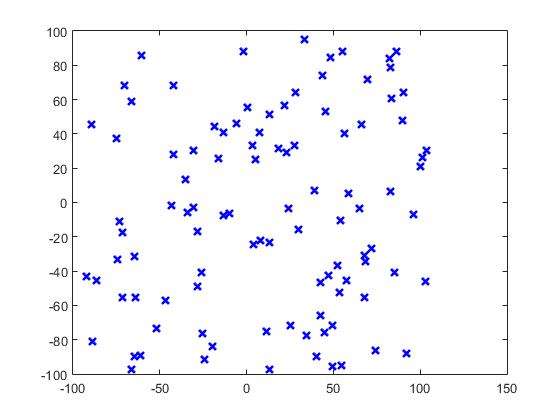
\includegraphics[width=8cm]{./g1.png}   
			\caption{Exemplo de primeira iteração}
			\label{fig:g1}
		\end{center}
	\end{figure}
	
	
\end{frame}

\begin{frame}
	
	\begin{figure}[h]
		\begin{center}
			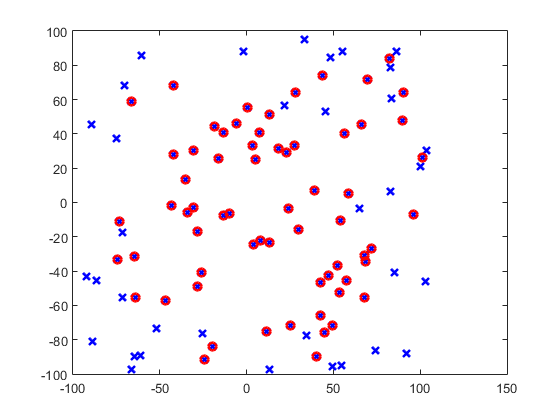
\includegraphics[width=8cm]{./g1_inter.png}   
			\caption{Exemplo de primeira iteração}
			\label{fig:g1_inter}
		\end{center}
	\end{figure}
	
	
\end{frame}

\begin{frame}
	
	\begin{figure}[h]
		\begin{center}
			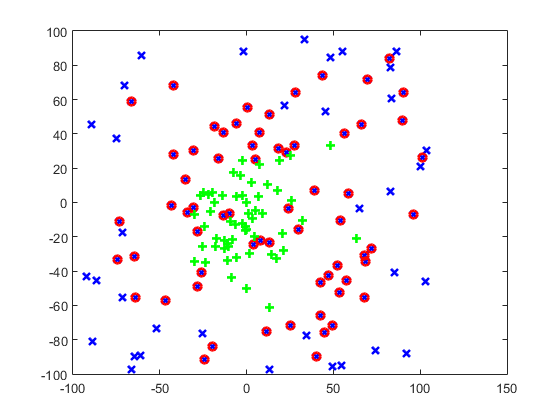
\includegraphics[width=8cm]{./g2.png}   
			\caption{Exemplo de primeira iteração}
			\label{fig:g2}
		\end{center}
	\end{figure}
	
	
\end{frame}
	
	



\mysection{Simplex}\label{sec:simplex}

\begin{frame}[t]{Simplex}
\begin{itemize}
\item Método de minimização multidimensional 
sem restrições
\item John A. Nelder e Roger Mead, 1965 ``The Computer Journal''.
\item Utiliza um Simplex para minimizar uma função de $n$ variáveis. 
\end{itemize}

\note{Também chamado de método Nelder-Mead}
\end{frame}

\begin{frame}[t]{Simplex}
\begin{itemize}
\pause
\item O que é um Simplex?\pause
\end{itemize}
\begin{figure}[h]
	\begin{center}	
		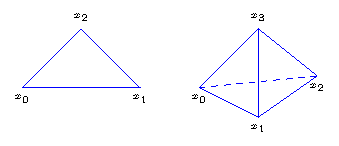
\includegraphics[width=10cm]{simplex/simplex.pdf}
		\caption{Exemplos de Simplex para $\mathbb{R}^2$ e $\mathbb{R}^3$.}
		\label{fig:simplex}
	\end{center}
\end{figure}
\note<1>{Mas a pergunta que não quer calar? O que é um simplex?}
\note<2>{Um Simplex é o menor politopo possível para um espaço de n variáveis. Como exemplo, vemos a figura \ref{fig:simplex}. Para $\mathbb{R}^2$ o menor politopo é um Triângulo, e para $\mathbb{R}^3$ é um Tetraedro.}
\note<3>{Exemplos de simplex}
\end{frame}

\begin{frame}[t]{Simplex}
\begin{itemize}
\item Método Generalista\pause
\item Não Precisa de cálculos complexos\pause
\item Considerado método de ordem $0$
\end{itemize}
\note<1,2>{Este é um método bem generalista que serve para diversos problemas pela sua facilidade, e por não necessitar de Gradientes e Hessianas, como veremos a seguir, é considerado um método de ordem 0.}
\note<3>{Então para facilitar a visualização, representação e entendimento, será explicado o método para $\mathbb{R}^2$}
\end{frame}

\begin{frame}[t]{Divisão do Método}
\pause
\begin{enumerate}
\item Ordenação \pause
\item Busca do Centróide\pause 
\item Reflexão \pause
\item Expansão\pause
\item Contração\pause
\item Encolhimento
\end{enumerate}
\note<7>{Serão explicados nos próximos slides}
\end{frame}

\begin{frame}[t]{Ordenação}
\begin{equation}
x_l=min(f(x_i))
\end{equation}
\begin{equation}
x_h=max(f(x_i)), x_i\neq x_l
\end{equation}
\begin{center}
		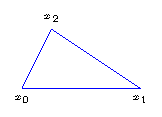
\includegraphics[width=4cm]{simplex/simplex3}
		\includegraphics<2>[width=4cm]{simplex/simplex2}
		
		
		\only<1>{{\usebeamercolor[fg]{caption name}Figura:} Pontos antes da ordenação}
		\only<2>{{\usebeamercolor[fg]{caption name}Figura:} Pontos após ordenação}
\end{center}
\note{\begin{itemize}
\item $x_h$ high
\item $x_l$ low
\item outro $x_s$ arbitrariamente
\end{itemize}}
\end{frame}

\begin{frame}[t]{Busca do Centróide}
\begin{equation}
c=\dfrac{x_l+x_s}{2}
\end{equation}
\begin{center}
		\includegraphics<1>[width=4cm]{simplex/simplex2}
		\includegraphics<2>[width=4cm]{simplex/centroide}
\end{center}
\note{encontra-se o centróide entre todos os pontos excluindo o $x_h$}
\end{frame}

\begin{frame}[t]{Reflexão}
\begin{equation}
x_r=c+\alpha(c-x_h)
\end{equation}
\begin{itemize}
\item $\alpha$=1
\end{itemize}
	
\begin{center}
		\includegraphics<1>[width=4cm]{simplex/centroide}
		\includegraphics<2>[width=4cm]{simplex/reflexao.pdf}
				
		\only<2>{{\usebeamercolor[fg]{caption name}Figura:} Reflexão}
\end{center}	
\end{frame}

\begin{frame}[t]{Reflexão}
\begin{itemize}
\item Se $f(x_l)<f(x_r)<f(x_s)$, $x_h$:=$x_c$\pause
\item Caso contrário, realizar alguma das próximas transformações 
\end{itemize}
\note<1>{Coeficiente de reflexão}
\end{frame}

\begin{frame}{Expansão}
\begin{itemize}
\item Se $f(x_r)<f(x_l)$
\end{itemize}
\begin{equation}
x_e=c+\gamma(x_r-c)
\end{equation}
\begin{itemize}
\item $\gamma$=2
\end{itemize}
\begin{figure}[H]
	\begin{center}	
		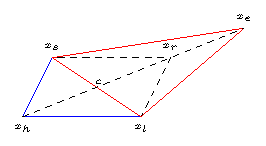
\includegraphics[width=6cm]{simplex/expansao.pdf}
		\caption{Expansão.}
		\label{fig:expansao}
	\end{center}
\end{figure}
\note{Coeficiente de expansão}
\end{frame}

\begin{frame}{Expansão}
\begin{itemize}
\item Se $f(x_r)<f(x_e)$, $x_h$:=$x_r$
\item Se $f(x_e)<f(x_r)$, $x_h$:=$x_e$
\end{itemize}
\note{pega o menor entre eles}
\end{frame}

\begin{frame}[t]{Contração}
\begin{itemize}
\item Se $f(x_r)\geq f(x_l)$
\end{itemize}
\begin{subnumcases}{x_c=}
   c+\beta(x_r-c) & Se $f(x_s)\leq f(x_r)<f(x_h)$ \label{positive}
   \\
   c+\beta(x_h-c) & Se $f(x_r)>f(x_h)$ \label{negative}
\end{subnumcases}
\begin{itemize}
\item $\beta$=$\frac{1}{2}$
\end{itemize}
\begin{figure}[h]
	\begin{center}	
		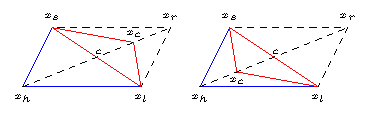
\includegraphics[width=8cm]{simplex/contracao.pdf}
		\caption{Representação das Contrações.}
		\label{fig:contracao}
	\end{center}
\end{figure}
\note<1>{Coeficiente de contração}
\end{frame}

\begin{frame}[t]{Contração}
\[
\text{Contração para fora}
  \begin{cases} 
    \text{Substituir $x_h$ por $x_c$} & \text{Se } f(x_c)\leq f(x_r) \\
   \text{Realizar encolhimento}       & \text{Se } f(x_c)>f(x_r)
  \end{cases}\]
  \[
  \text{Contração para dentro}
  \begin{cases} 
   \text{Substituir $x_h$ por $x_c$} & \text{Se } f(x_c)<f(x_h) \\
   \text{Realizar encolhimento}       & \text{Se } f(x_c)\geq f(x_h)
  \end{cases}
\]
\end{frame}


\begin{frame}[t]{Encolhimento}
\begin{subequations}
\begin{align}
x_s:=x_s+\delta (x_s-x_l)\\
x_h:=x_h+\delta (x_h-x_l)
\end{align}
\end{subequations}
\begin{itemize}
\item $\delta$=$\frac{1}{2}$
\end{itemize}
\begin{figure}[h]
	\begin{center}	
		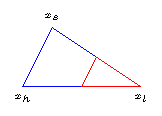
\includegraphics[width=4cm]{simplex/encolher.pdf}
		\caption{Encolhimento.}
		\label{fig:encolher}
	\end{center}
\end{figure}
\note{O encolhimento é muito raro de acontecer e é usado para quando todas as outras transformações anteriores resultam em pontos cujo valor correspondente na função é pior que os anteriores. O que só acontece em casos específicos. Exemplo de caso pode ser visto um extrato da publicação original de 1965
}
\end{frame}

\begin{frame}[t]{Encolhimento}
\begin{quote}
``A failed contraction is much rarer, but can occur when a valley is curved and one point of the simplex is much farther from the valley bottom than the others; contraction may then cause the reflected point to move away from the valley bottom instead of towards it. Further contractions are then useless. The action proposed contracts the simplex towards the lowest point, and will eventually bring all points into the valley.''
\end{quote}
\note{blablablabla....}
\end{frame}

\begin{frame}[t]{Critérios de Parada}
\begin{enumerate}\pause
\item Iterações\pause
\item Raio da circunferência circunscrita
\item<4-5> Desvio Padrão dos $f(x)$
\end{enumerate}
\begin{center}
		\includegraphics<3>[width=5cm]{simplex/parada.pdf}
		\includegraphics<4-5>[width=8cm]{simplex/desviopadrao.pdf}
				
		\only<3>{{\usebeamercolor[fg]{caption name}Figura:} Circunferência circunscrita ao simplex.}
		\only<4>{{\usebeamercolor[fg]{caption name}Figura:} Desvio padrão}
		\only<5>{{\usebeamercolor[fg]{caption name}} Onde $\sigma$=$\sqrt{\frac{\sum_i^n(y_i-\overline{y})^2}{n}}$}
\end{center}
\note<1>{Foram utilizados 3 critérios de parada nesse método}
\note<4>{Cálculo do desvio utilizando três dados por vez. Cada vértice do triângulo a partir da fórmula a seguir}
\note<5>{Quando o desvio chega a zero significa que a superfície se comporta como um plano que não possui mínimo.}
\end{frame}


\mysection{Interface Gráfica}\label{sec:gui}

bla bla bla

\mysection{Resultados e Discussão}\label{sec:resultados}
Após implementados todos os métodos, foram testados para realizar a minimização quadrática segundo o enunciado:\\

\fbox{\begin{minipage}{34em}
	
	\textbf{2.)} A resposta ao impulso unitário de um sistema foi medida em laboratório,resultando na tabela abaixo\vspace{10pt}
	
	\begin{tabular}{|c||c|c|c|c|c|c|c|c|c|c|}
		\hline
		t$\rightarrow$ & 0.50 & 1.00&1.50 &2.00 &2.50 &3.00 &3.50 &4.00 &4.50 &5.00\\
		\hline
		m(t)$\rightarrow$ & 1.65 & -1.30 &0.50 &-0.10 &-0.15 &0.15 &-0.05 &0.05 &0.01 &0.00\\
		\hline
	\end{tabular}\vspace{10pt}
	
	Deseja-se atribuir a este sistema um modelo LIT caracterizado por \linebreak$H(s)=\omega_n^2/(s^2+2\zeta\omega_ns+\omega_n^2)$ cuja resposta ao impulso unitário é $h(t)=(\omega_n^2/\omega_d)e^{-\zeta\omega_nt}sen(\omega_dt)$, onde $\omega_d=\omega_n\sqrt{1-\zeta^2}$. Pelo método dos mínimos quadrados, encontrar a melhor estimativa para $\zeta$ e $\omega_n$, usando (a) 03 das amostras acima,(b) 05 delas, (c) todas. Comente os resultados obtidos.
	
\end{minipage}}

\vspace{20pt}

Fizemos as operações de encontrar a função objetivo usando os dados $t$ e $m(t)$ da tabela e $h(t)$ e o método mostrado na seção \ref{sec:min_quad}, para 3, 5 e 10 amostras.

Cada uma das três funções objetivo foram testadas em todos os métodos de minimização vetorial implementados durante a realização da matéria de Introdução a Otimização, tantos os métodos ``nobres" (Newton e Gradiente por exemplo) quanto nos métodos ``pobres" mostrados neste documento. Infelizmente, todos os métodos ``nobres" possuíram grande dificuldade, obtendo iterações que duravam minutos tornando assim impossível de computar a minimização.

Nos métodos pobres, O algoritmo genético utilizado neste trabalho mostrou-se eficiente para funções bem comportadas (quadráticas por exemplo), mas em funções menos comportadas, como a função objetivo para 3, 5 e 10 amostras, obteve semelhantemente dificuldades na hora de computar a minimização. Por isso tentou-se utilizar somente duas amostras, e mesmo assim as iterações demoravam dezenas de minutos cada, devido a explosão combinatória na hora da "reprodução".\newpage

A seguir vemos os resultados obtidos para o simplex. As figuras \ref{fig:p_iter_3}, \ref{fig:p_iter_5} e \ref{fig:p_iter_10} mostram a convergência do método e as figuras \ref{fig:p_impulse_3}, \ref{fig:p_impulse_5} e \ref{fig:p_impulse_10}, mostram a resposta ao impulso unitário do sistema proposto pela minimização.\vspace{10pt}\\
Para 3 amostras os valores de $\omega_n$ e $\zeta$ encontrados foram  4.8207 e 0.30037\\
Para 5 amostras os valores de $\omega_n$ e $\zeta$ encontrados foram  2.0521 e 0.30193\\
Para 10 amostras os valores de $\omega_n$ e $\zeta$ encontrados foram  4.9804 e 0.26358\\\\
Fim pelo número de Iterações\\
Iterações: 120/200\\
Tempo de simulação: 5.518\\
Coordenadas do mínimo: (4.8207,0.30037,0.0019568)\\\\
Fim pelo tamanho do Raio da Circunferência Circunscrita\\
Iterações: 69/200\\
Tempo de simulação: 3.628\\
Coordenadas do mínimo: (2.0521,0.30193,0.42709)\\\\
Fim pelo tamanho do Raio da Circunferência Circunscrita\\
Iterações: 71/200\\
Tempo de simulação: 3.837\\
Coordenadas do mínimo: (4.9804,0.26358,0.011948)\\





\twocolumn
\begin{figure}[H]
	\begin{center}	
		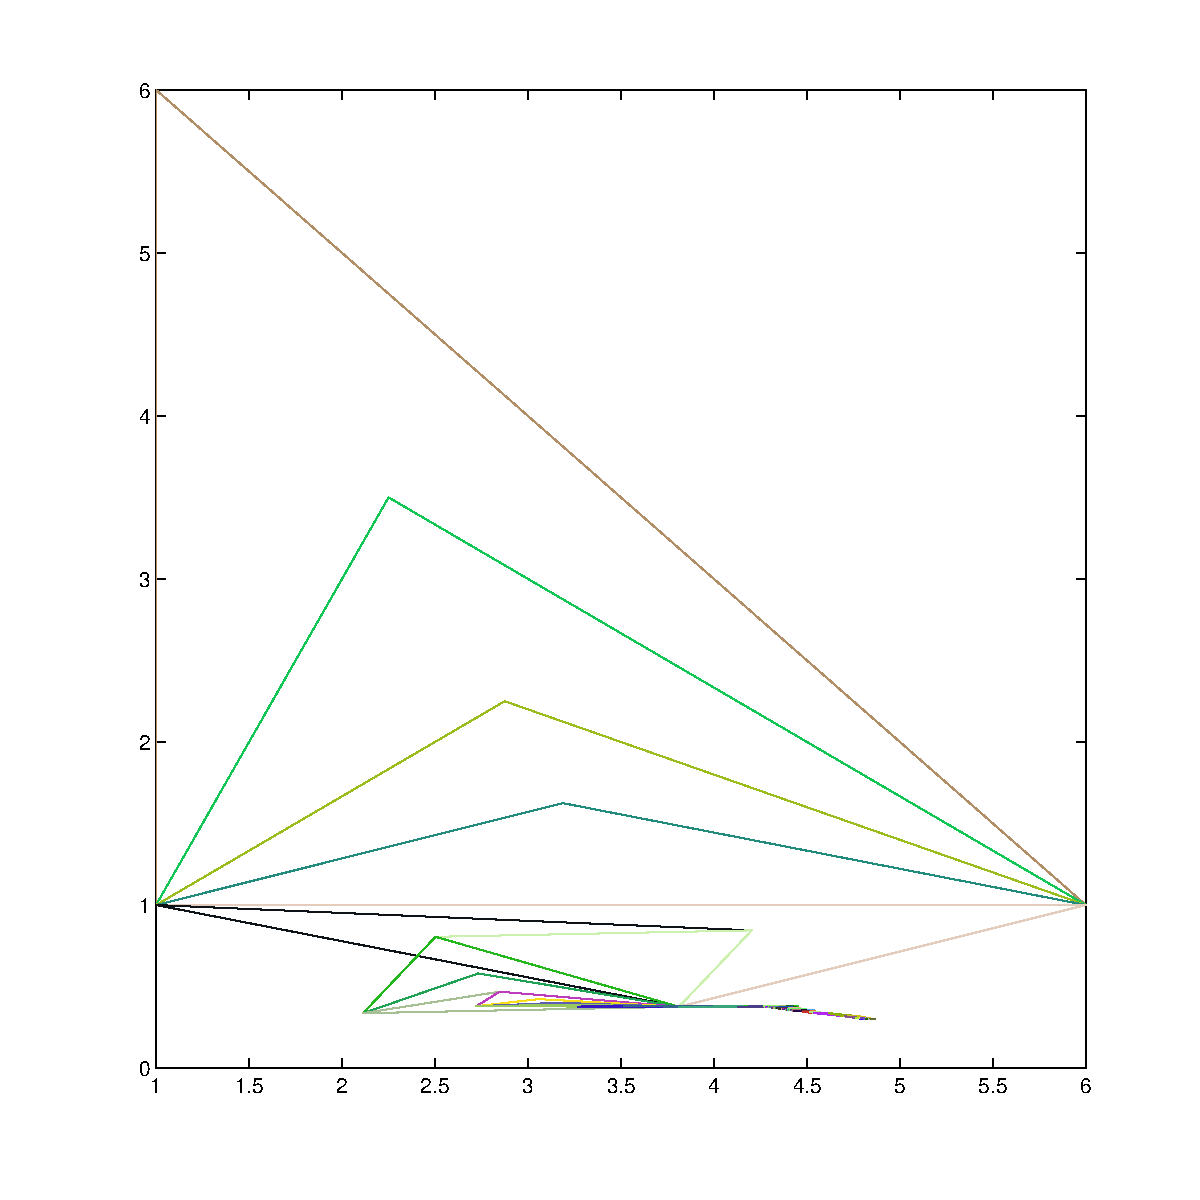
\includegraphics[width=6cm]{Plots/p_iter_3.pdf}
		\caption{Convergência para 3 amostras}
		\label{fig:p_iter_3}
	\end{center}
\end{figure}

\begin{figure}[H]
	\begin{center}	
		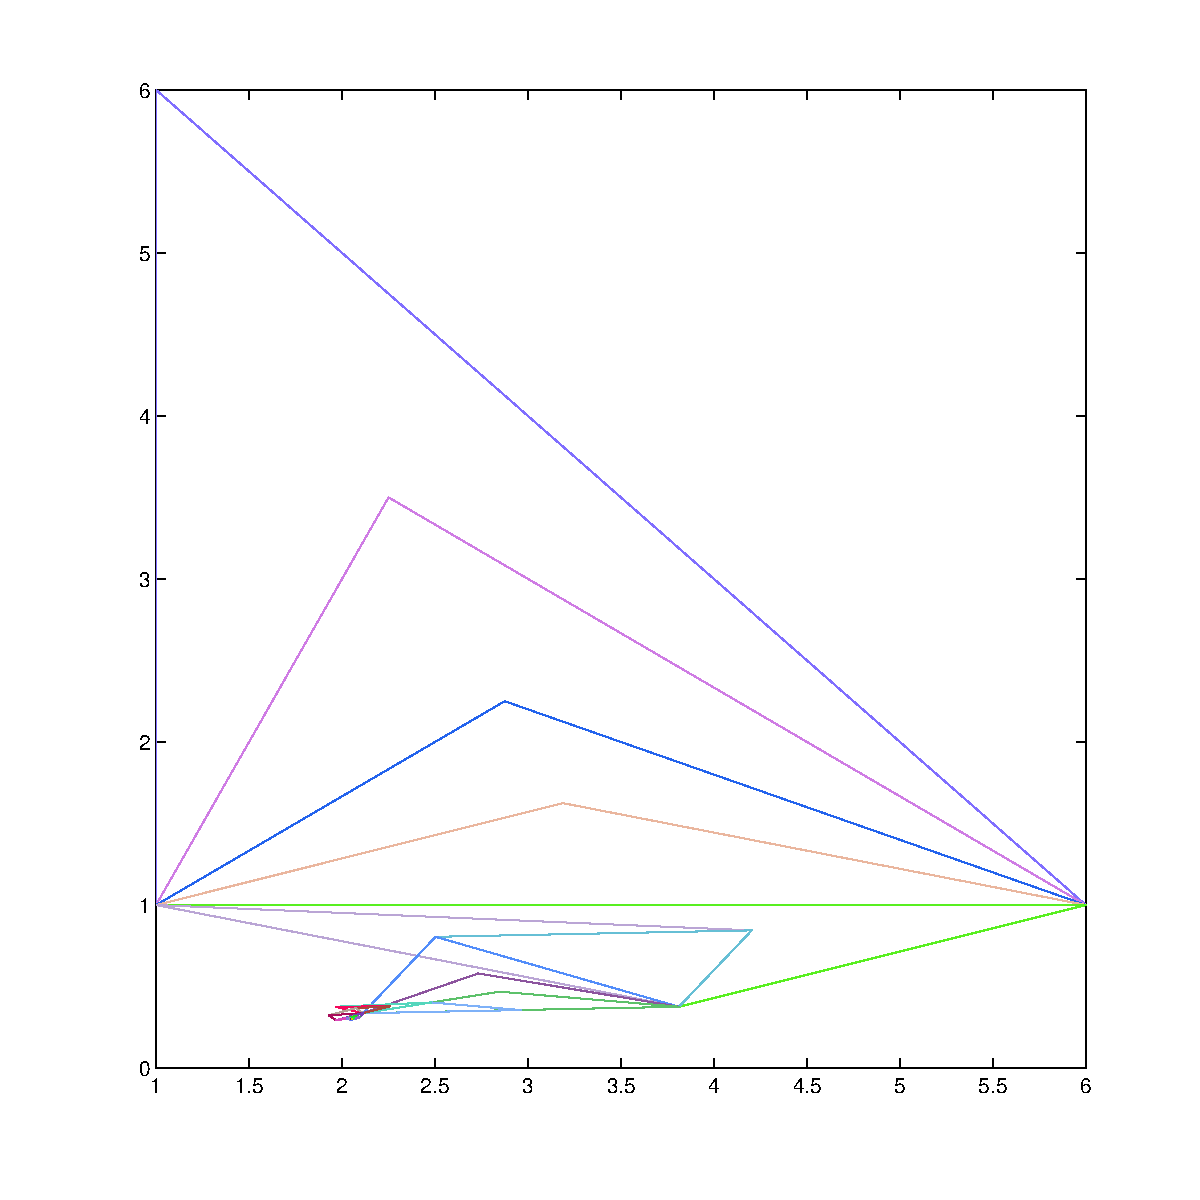
\includegraphics[width=6cm]{Plots/p_iter_5.pdf}
		\caption{Convergência para 5 amostras}
		\label{fig:p_iter_5}
	\end{center}
\end{figure}

\begin{figure}[H]
	\begin{center}	
		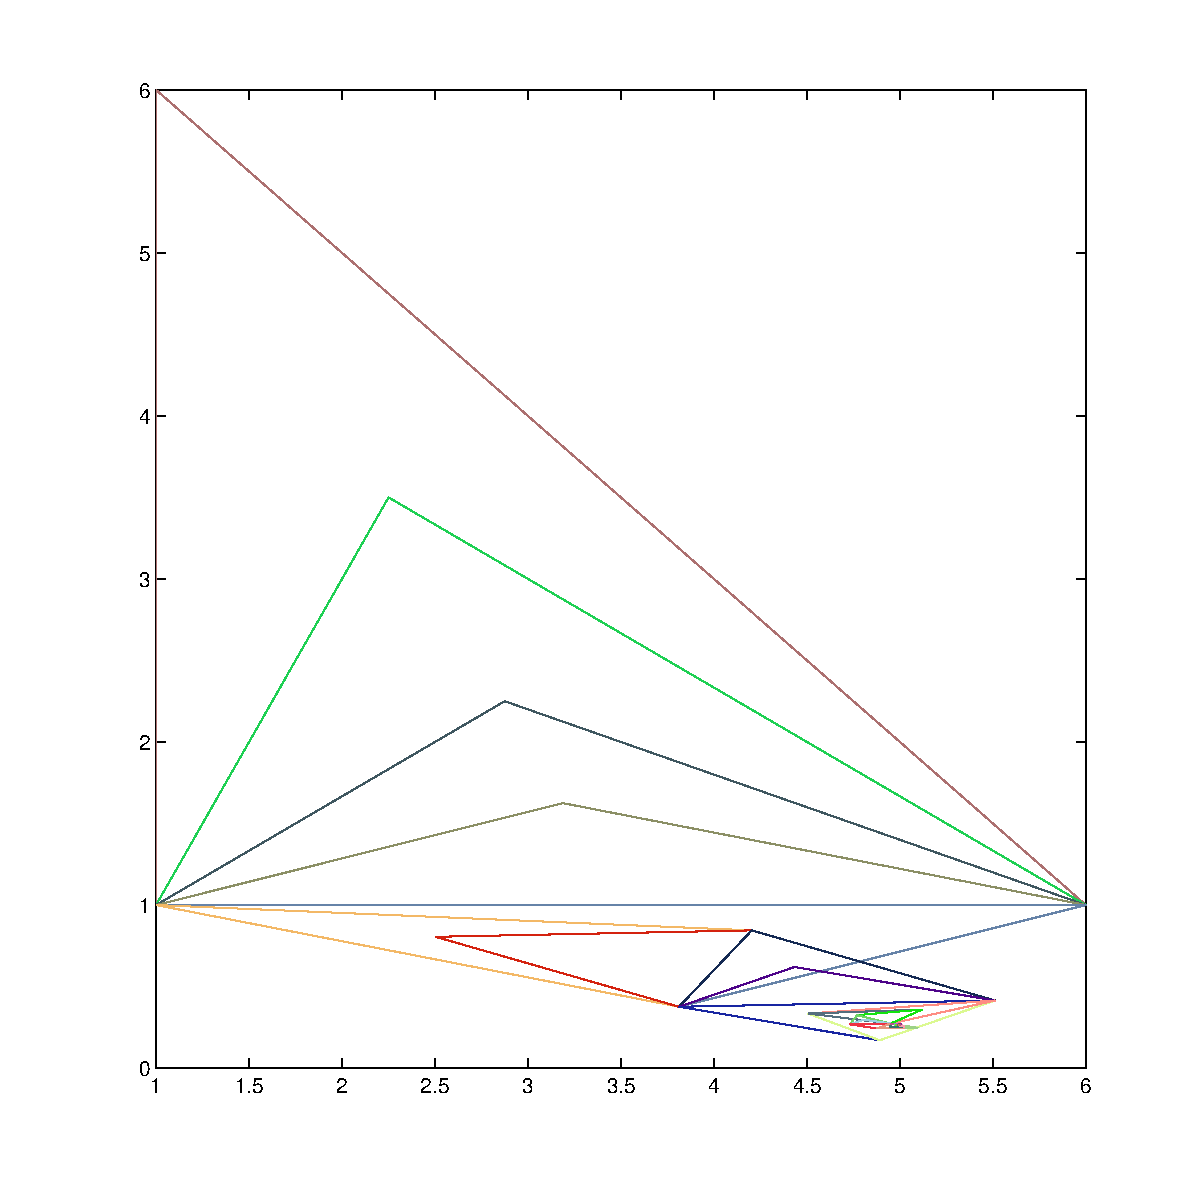
\includegraphics[width=6cm]{Plots/p_iter_10.pdf}
		\caption{Convergência para 10 amostras}
		\label{fig:p_iter_10}
	\end{center}
\end{figure}



\begin{figure}[H]
	\begin{center}	
		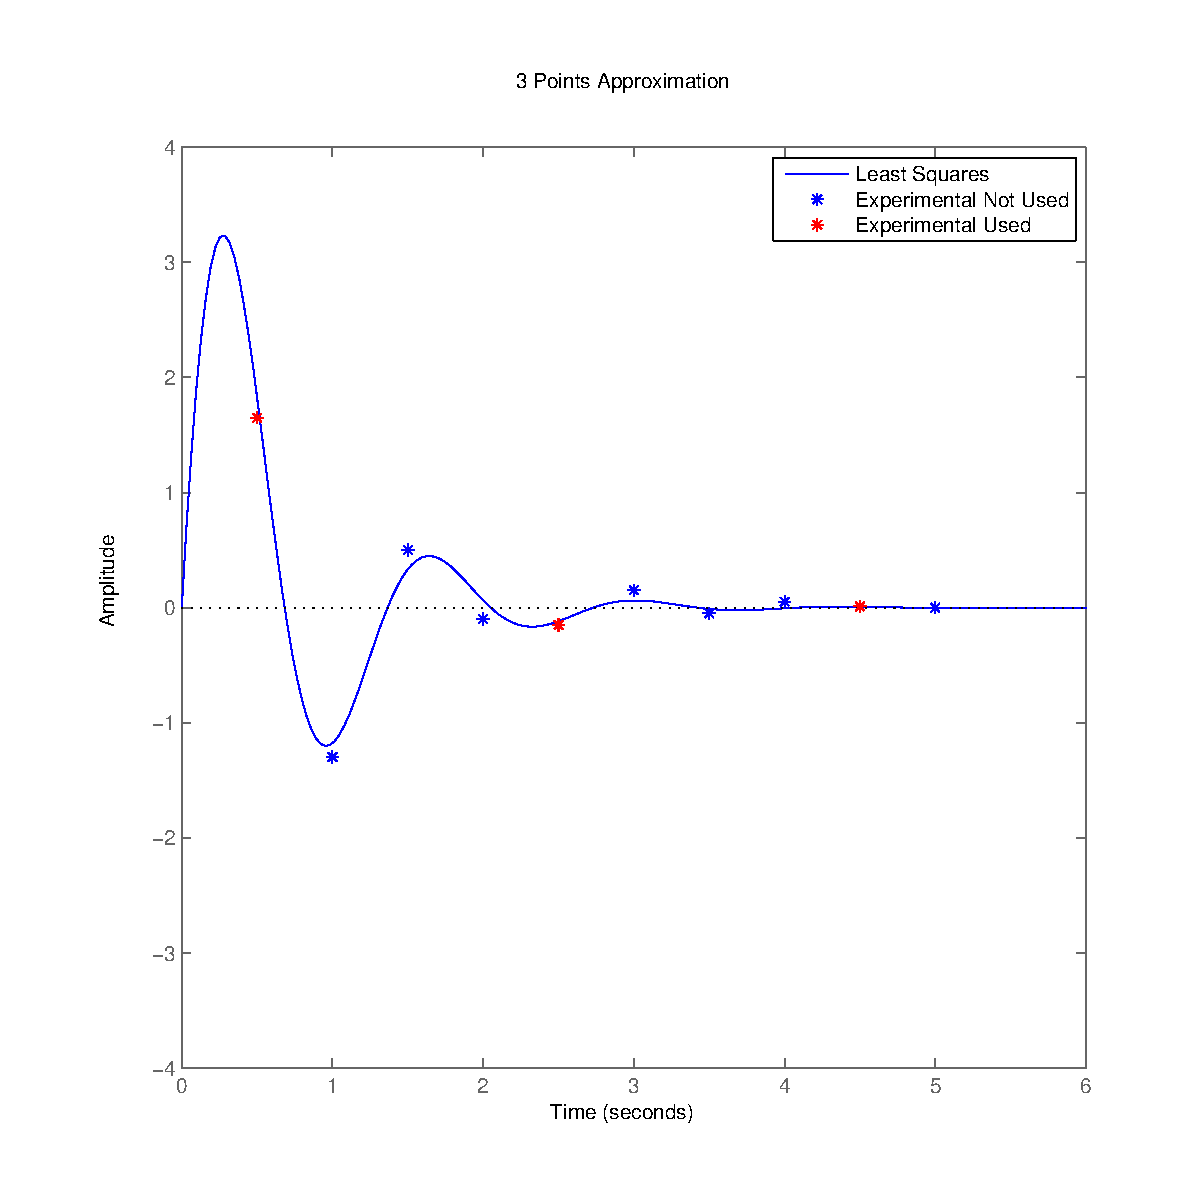
\includegraphics[width=6cm]{Plots/p_impulse_3.pdf}
		\caption{Resposta do impulso (3 amostras)}
		\label{fig:p_impulse_3}
	\end{center}
\end{figure}

\begin{figure}[H]
	\begin{center}	
		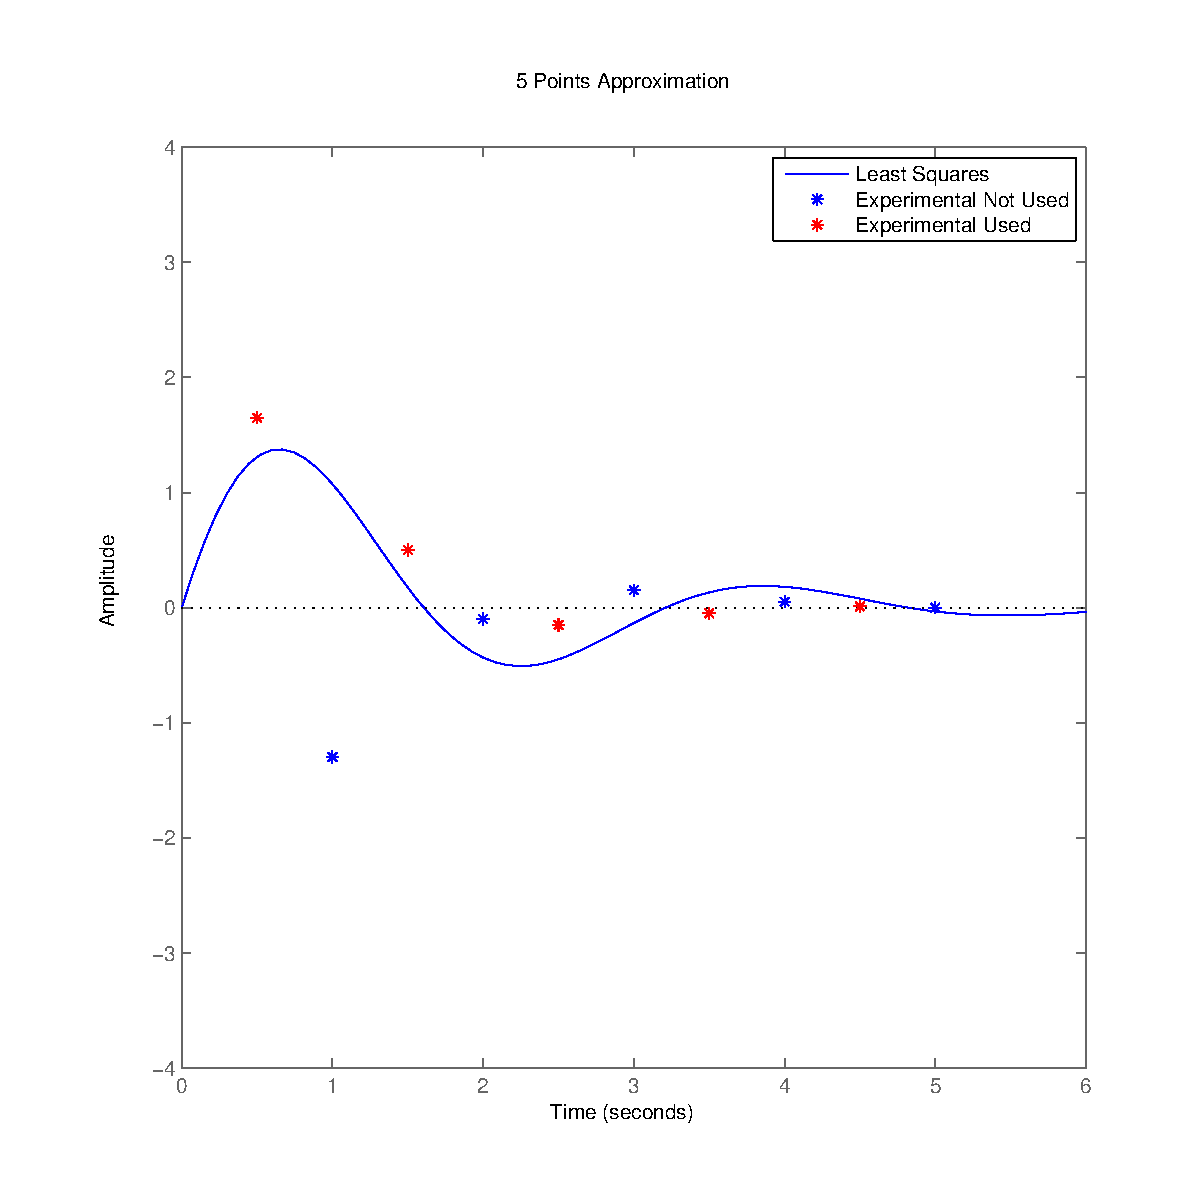
\includegraphics[width=6cm]{Plots/p_impulse_5.pdf}
		\caption{Resposta do impulso (5 amostras)}
		\label{fig:p_impulse_5}
	\end{center}
\end{figure}

\begin{figure}[H]
	\begin{center}	
		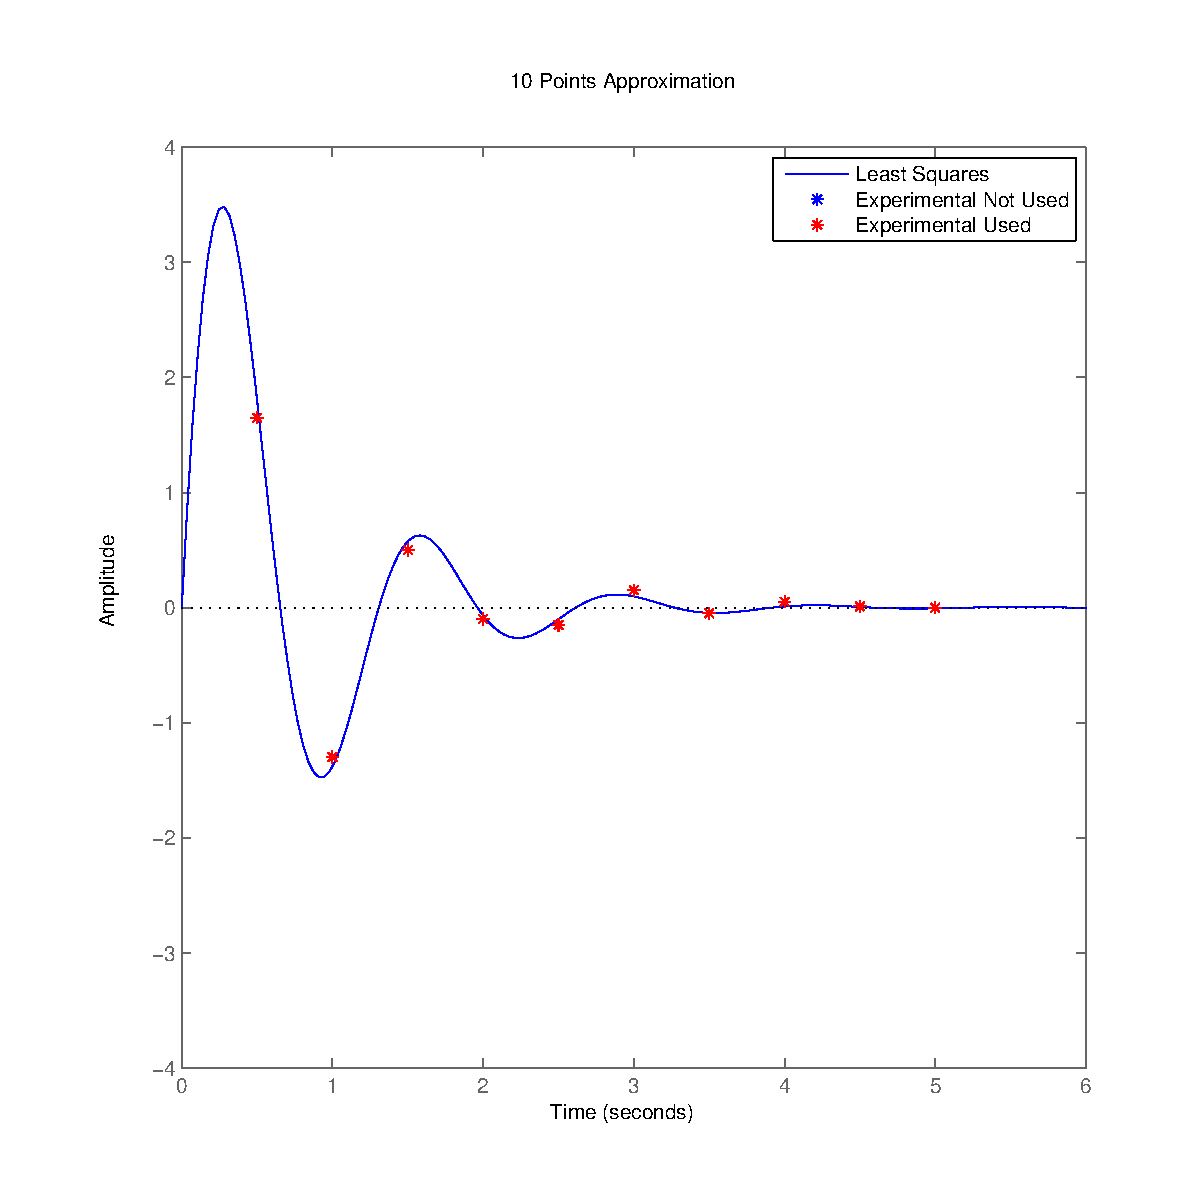
\includegraphics[width=6cm]{Plots/p_impulse_10.pdf}
		\caption{Resposta do impulso (10 amostras)}
		\label{fig:p_impulse_10}
	\end{center}
\end{figure}
\onecolumn
\newpage



\mysection{Conclusão}

bla bla bla
	

\bibliographystyle{plain}
\bibliography{bibliografia}

\end{document}